\subsection{Localized-growth benchmarks: weighted particles, resampling, and branching}
\label{sec:branch_vs_weight}
To compare particle-level realizations of the reaction operator, we first consider the
scalar localized-growth problem
\begin{equation}
\partial_t u=D\Delta u+r(\mathbf x)u,
\qquad
r(\mathbf x)=\lambda G(\mathbf x)-\beta,
\qquad
G_\sigma(\mathbf x)=\exp\!\left(-\frac{|\mathbf x-\mathbf x_0|_{\mathbb T}^2}{2\sigma^2}\right),
\label{equ:loc_growth}
\end{equation}
with \(D=0.05\), \(\lambda=8\), \(\beta=1\), \(\sigma=0.5\), \(\mathbf x_0=0\),
\(u_0=1+G/2\), \(T=1\), \(\tau=2\times10^{-3}\), \(K=16\), and
\(N_0=2\times10^4\).  The deterministic reference is a Fourier Strang split-step
solution on a \(256^2\) grid.  The diagnostic region is the fixed growth set
\(\Omega_{\rm grow}=\{G_\sigma\ge 0.5\}\).

The weighted baselines use the same transport, the same initial particles, and the same
finite-measure normalization as the branching runs.  The resampled baselines use
systematic resampling.  In the ESS-triggered policy we resample when the global
normalized ESS falls below \(0.5\); in the every-step policy used below for the switching
test we resample after every reaction update.  For a finite measure, resampling draws
\(N_0\) indices with probabilities proportional to the current weights and then resets all
particles to the common weight \(\bar w=(\sum_i w_i)/N_0\), so the represented total mass
is preserved exactly by the resampling operation.

The final-time comparison is summarized in Table~\ref{tab:bw}.  In this table,
\[
\mathrm{nESS}
=
\frac{(\sum_i w_i)^2}{N_{\rm rep}\sum_i w_i^2},
\]
where \(N_{\rm rep}\) is the number of particles in the reported representation at
\(T\); hence \(\mathrm{nESS}=1\) for equal-weight branching.  For a diagnostic region
\(B\), we use the same normalized formula restricted to particles in \(B\) and denote it
by \(\mathrm{nESS}(B)\).  The table also reports the actual number \(N_B\) of
particles in \(\Omega_{\rm grow}\) for the equal-weight representations; after
resampling this is the duplicated local particle count, while for branching it is the
reaction-generated local particle count.  The peak error is the absolute peak-height
error,
\[
E_{\rm peak}
=
\left|
\|\widetilde u^{N,K}(T)\|_{L^\infty}
-
\|u_{\rm ref}(T)\|_{L^\infty}
\right|.
\]
The raw weighted method develops the expected localized weight degeneracy: its
normalized ESS is \(0.021\), the maximum-to-mean weight ratio is \(133\), and the
relative \(L^2\) error is \(0.269\pm0.041\).  ESS-triggered resampling reduces the
weight degeneracy and improves the error, but it keeps a fixed active population.
Equal-weight branching instead represents the same reaction-induced mass growth as
particle count.  At the same initial budget, the Poisson kernel gives
\(0.062\pm0.035\), while the minimum-variance kernel gives \(0.033\pm0.011\),
consistent with its smaller conditional offspring variance.  The corresponding
reconstructed fields and error histories are shown in Fig.~\ref{fig:bw_snap_l2}; the raw
weighted reconstruction under-resolves the peak, whereas ESS resampling and
minimum-variance branching recover it more accurately.

For the cost comparison, we denote the active particle count by
\(
N_{\rm act}(t)=|\mathcal I(t)|
\)
and use the integrated particle-step count
\(
W_{\rm p}=\sum_{n=0}^{T/\tau}N_{\rm act}(t_n).
\)
For weighted and resampled weighted particles \(N_{\rm act}(t)\) is fixed by the chosen
particle budget, whereas for branching it is generated by the integer reaction
realization.  The cost controls in Table~\ref{tab:bw_cost} separate the representation
effect from a simple increase in particle budget.  At matched work
\(W_{\rm p}\approx1.9\times10^7\), ESS-triggered systematic resampling gives
\(0.047\pm0.012\), while minimum-variance branching gives \(0.033\pm0.011\).  The larger
\(1.3\times10^5\)-particle ESS run is more accurate, but it uses about
\(6.6\times10^7\) particle steps.  Thus the comparison should be read as a controlled
representation result, not as a claim that branching dominates every possible resampling
strategy at every budget.

\begin{table}[t]
\centering
\small
\caption{Stationary localized-growth benchmark at \(T=1\), with common transport and
\(N_0=2.0\times10^4\).  Weighted rows report global normalized ESS, local normalized
ESS in \(\Omega_{\rm grow}\), and max:mean weight ratio.  Equal-weight rows report the
actual local particle count \(N_B\) in \(\Omega_{\rm grow}\).  Values are means over the
reported seeds, with standard deviations shown for the error columns.}
\label{tab:bw}
\begin{tabular}{l c c c c c c}
\toprule
method & rel. \(L^2\) error & nESS & local nESS & max:mean \(w\) & local \(N_B\) & \(E_{\rm peak}\) \\
\midrule
weighted & \(0.269\pm0.041\) & 0.021 & 0.431 & 133 & -- & \(149\pm94\) \\
weighted + ESS & \(0.073\pm0.033\) & 0.56 & 0.882 & 3.1 & \(9.27\times10^3\) & \(37\pm34\) \\
Poisson br. & \(0.062\pm0.035\) & 1 & -- & -- & \(1.13\times10^5\) & \(31\pm24\) \\
min.-var. br. & \(\mathbf{0.033\pm0.011}\) & 1 & -- & -- & \(\mathbf{1.09\times10^5}\) & \(\mathbf{12.7\pm7.0}\) \\
\bottomrule
\end{tabular}
\end{table}

\begin{table}[t]
\centering
\caption{Cost and large-budget controls for the stationary localized-growth benchmark.
Here \(W_{\rm p}=\sum_n N_{\rm act}(t_n)\) is the integrated particle-step count.}
\label{tab:bw_cost}
\begin{tabular}{l c c c}
\toprule
method & initial budget & \(W_{\rm p}\) & rel. \(L^2\) error \\
\midrule
weighted & \(6.0\times10^4\) & \(3.0\times10^7\) & \(0.151\pm0.021\) \\
weighted & \(1.3\times10^5\) & \(6.6\times10^7\) & \(0.089\pm0.018\) \\
weighted + ESS & \(3.8\times10^4\) & \(1.9\times10^7\) & \(0.047\pm0.012\) \\
weighted + ESS & \(1.3\times10^5\) & \(6.6\times10^7\) & \(0.028\pm0.006\) \\
min.-var. br. & \(2.0\times10^4\) & \(\mathbf{1.9\times10^7}\) & \(\mathbf{0.033\pm0.011}\) \\
\bottomrule
\end{tabular}
\end{table}

\begin{figure}[t]
\centering
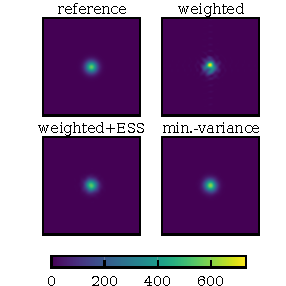
\includegraphics[width=0.4\linewidth]{figure/snapshots_final.pdf}\quad
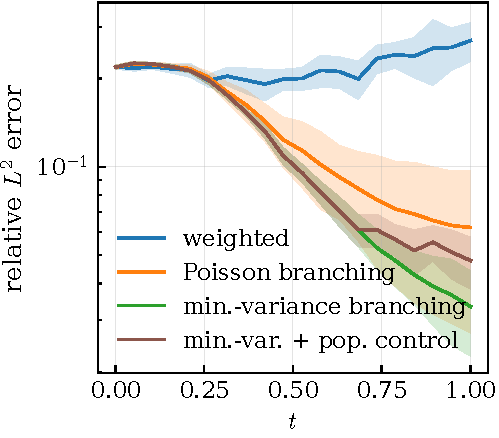
\includegraphics[width=0.4\linewidth]{figure/l2_vs_t.pdf}
\caption{Stationary localized-growth benchmark.  Left: final-time reconstructed fields
at \(T=1\) for the deterministic reference, raw weighted particles, ESS-resampled
weighted particles, and minimum-variance branching, all with \(N_0=2.0\times10^4\).
Right: relative \(L^2\) error versus time for the same initial budget.  Raw weighting
under-resolves the localized peak, while ESS resampling and minimum-variance branching
reduce the error; quantitative final-time diagnostics are reported in
Table~\ref{tab:bw}.  The matched-work comparison is reported separately in
Table~\ref{tab:bw_cost}.}
\label{fig:bw_snap_l2}
\end{figure}

\paragraph{Switching localized growth.}
We further test the representation comparison with a growth region that switches from
\(\mathbf x_A=(-1.2,0)\) to \(\mathbf x_B=(1.2,0)\) at mid-time:
\begin{equation}
\partial_tu=D\Delta u+r(t,\mathbf x)u,
\qquad
r(t,\mathbf x)=\lambda\bigl[(1-s(t))G_\sigma(\mathbf x;\mathbf x_A)+s(t)G_\sigma(\mathbf x;\mathbf x_B)\bigr]-\beta,
\qquad
s(t)=\frac12\left(1+\tanh\frac{t-T/2}{\delta}\right).
\label{equ:switch}
\end{equation}
Here \(u_0\equiv1\), \(D=0.02\), \(\lambda=10\), \(\beta=0.1\), \(\sigma=0.25\),
\(T=1.2\), \(\delta=0.04\), \(\tau=10^{-3}\), \(K=48\), and
\(N_0=2\times10^4\).  The reference field \(u_{\rm ref}\) is computed by a deterministic
Fourier pseudospectral solver on a \(512\times512\) collocation grid.  We use the
half-height sets
\[
B_A=\{G_\sigma(\mathbf x;\mathbf x_A)\ge 0.5\},
\qquad
B_B=\{G_\sigma(\mathbf x;\mathbf x_B)\ge 0.5\}
\]
as the local diagnostic regions.
The second-stage region \(B_B\) is the discriminating diagnostic.  Table~\ref{tab:switch}
shows that ESS-triggered resampling gives the smallest error in the first-stage region
\(B_A\), where the fixed particle budget has been concentrated before the switch, but it
has larger error in the later region \(B_B\).  Branching gives lower
\(B_B\) error under the same initial budget, while increasing the active population
through the reaction step.  In this switching run the two branching kernels are close:
the Poisson kernel has the smallest mean global and \(B_B\) errors, while the
minimum-variance kernel has the smaller \(B_B\) seed-to-seed spread.  We show the
minimum-variance kernel in Fig.~\ref{fig:switch} because it is the default low-variance
branching representation used elsewhere.

The lineage diagnostic in Table~\ref{tab:switch_anc} supports the mechanism.  Just
before the source moves, ESS-triggered resampling has reduced the global number of
distinct surviving initial ancestors to about \(1.35\times10^4\), compared with about
\(1.89\times10^4\) for branching.  In the future growth region \(B_B\), ESS resampling
retains \(92\pm16\) distinct ancestors, while minimum-variance branching retains
\(123\pm11\), close to the raw weighted background count.  Thus global resampling has
already committed part of the fixed particle budget to the old region, whereas branching
retains background lineages and then creates equal-weight particles when the new growth
region turns on.

\begin{table}[t]
\centering
\caption{Switching-growth benchmark at \(T=1.2\) (eight seeds): relative \(L^2\) errors globally and in the first- and second-stage regions.}
\label{tab:switch}
\begin{tabular}{l c c c }
\toprule
method & global \(L^2\) & \(B_A\) \(L^2\) & \(B_B\) \(L^2\)   \\
\midrule
weighted & \(0.900\pm0.048\) & \(1.014\pm0.120\) & \(0.690\pm0.039\)  \\
weighted + resample (ESS) & \(0.288\pm0.025\) & \(\mathbf{0.162\pm0.027}\) & \(0.297\pm0.038\) \\
weighted + resample (every step) & \(0.271\pm0.062\) & \(0.234\pm0.087\) & \(0.226\pm0.107\)  \\
Poisson branching & \(\mathbf{0.199\pm0.045}\) & \(0.183\pm0.063\) & \(\mathbf{0.168\pm0.067}\)  \\
minimum-variance branching & \(0.203\pm0.051\) & \(0.170\pm0.136\) & \(0.174\pm0.022\)   \\
\bottomrule
\end{tabular}
\end{table}

\begin{table}[t]
\centering
\caption{Lineage diagnostic for the switching-growth benchmark just before the switch,
\(t=0.599\).  The table reports distinct initial ancestors among all active particles
and inside the future growth region \(B_B\).}
\label{tab:switch_anc}
\begin{tabular}{l c c}
\toprule
method & global distinct ancestors & distinct ancestors in \(B_B\) \\
\midrule
weighted & \(2.00\times10^4\) & \(132\pm14\) \\
weighted + resample (ESS) & \((1.35\pm0.17)\times10^4\) & \(92\pm16\) \\
weighted + resample (every step) & \((1.27\pm0.09)\times10^4\) & \(97\pm21\) \\
Poisson branching & \((1.89\pm0.003)\times10^4\) & \(128\pm9\) \\
minimum-variance branching & \((1.89\pm0.002)\times10^4\) & \(123\pm11\) \\
\bottomrule
\end{tabular}
\end{table}

\begin{figure}[t]
\centering
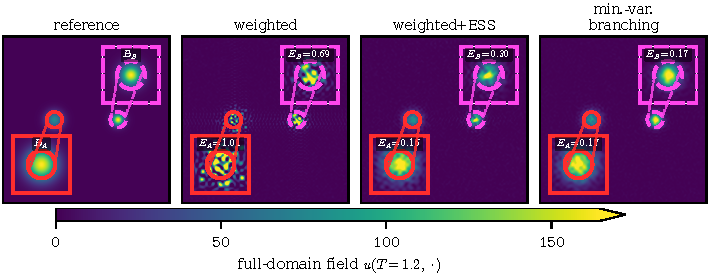
\includegraphics[width=0.8\linewidth]{figure/switch_snapshots_magnifier_4x1.pdf}
\caption{Switching-growth benchmark at \(T=1.2\), after the source has moved from
\(\mathbf x_A\) to \(\mathbf x_B\).  The panels compare the deterministic reference,
raw weighted particles, ESS-resampled weighted particles, and minimum-variance
branching.  Each panel shows the full-domain reconstruction together with magnified
views of the old growth region \(B_A\) and the new growth region \(B_B\).  The insets
visualize the mechanism quantified in Table~\ref{tab:switch}: ESS resampling is most
accurate in the old region \(B_A\), while branching gives lower error in the later
region \(B_B\) under the same initial budget.}
\label{fig:switch}
\end{figure}
